\documentclass[a4paper,12pt]{article}
\usepackage[utf8]{inputenc}
\usepackage[T1]{fontenc}
\usepackage[english]{babel}
\usepackage{geometry}
\usepackage{graphicx}
\usepackage{hyperref}
\usepackage{array}
\usepackage{tikz}
\usepackage{caption}
\usepackage{float}
\usepackage{needspace} 
\geometry{margin=2.5cm}

\usepackage{listings}
\lstset{
  basicstyle=\ttfamily\small,
  breaklines=true,
  frame=single
}

\title{ARC/DIR Format and \texttt{arcdir\_tool}\\Complete Technical Documentation}
\author{}
\date{\today}

\begin{document}
\maketitle
\tableofcontents
\newpage

\section{Introduction}

This document provides a structured technical description of the paired \texttt{.arc}/\texttt{.dir} archive format
and the \texttt{arcdir\_tool} utility used for extracting, packing, and managing archive data.
It covers command-line syntax, internal algorithms, binary file structures, alignment rules, and practical examples.

The utility is implemented in C, ensuring:  
\needspace{3\baselineskip}
\begin{itemize}
  \item High performance through direct file I/O;
  \item Cross-platform compatibility (Windows and POSIX systems);
  \item Deterministic behavior for identical input data.
\end{itemize}

\section{Concept Overview}

The archive format consists of two interrelated files:  
\needspace{3\baselineskip}
\begin{itemize}
  \item \texttt{.arc} --- a sequential concatenation of raw file data;
  \item \texttt{.dir} --- an index containing metadata such as file offsets, sizes, and paths.
\end{itemize}

The \texttt{.dir} file functions as a structured index for \texttt{.arc}, mapping file paths to their offsets and sizes.

\section{System Architecture}

\begin{table}[H]
\centering
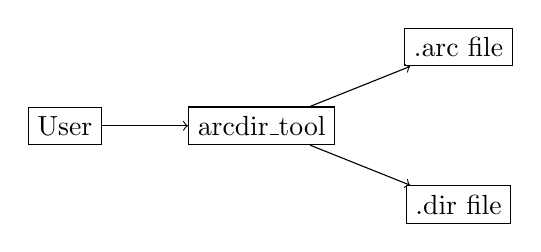
\begin{tikzpicture}[node distance=2.5cm, auto]
  \node[draw, rectangle] (user) {User};
  \node[draw, rectangle, right of=user] (tool) {arcdir\_tool};
  \node[draw, rectangle, right of=tool, yshift=1cm] (arc) {.arc file};
  \node[draw, rectangle, right of=tool, yshift=-1cm] (dir) {.dir file};

  \draw[->] (user) -- (tool);
  \draw[->] (tool) -- (arc);
  \draw[->] (tool) -- (dir);
\end{tikzpicture}
\caption{Overall architecture of \texttt{arcdir\_tool}}
\end{table}
\newpage

\section{Program Execution Flow}

The execution flow of \texttt{arcdir\_tool} can be described as a linear sequence of operations:

\needspace{15\baselineskip}
\begin{enumerate}
  \item Parse command-line arguments and identify the mode: \texttt{EXTRACT}, \texttt{PACK}, or \texttt{PACK\_BIN}.
  \item \textbf{EXTRACT mode:}
    \begin{itemize}
      \item Open ARC and DIR files in read mode;
      \item Read DIR entries sequentially;
      \item Apply optional path redirection rules;
      \item Write file data to the corresponding output paths.
    \end{itemize}
  \item \textbf{PACK / PACK\_BIN modes:}
    \begin{itemize}
      \item Recursively scan the specified directories and files;
      \item Apply extension filter (\texttt{.bin} for PACK\_BIN mode);
      \item Sort all discovered paths lexicographically;
      \item Write DIR entries and sequentially place file data in ARC;
      \item Apply padding for path strings (4-byte alignment) and file data (32-byte alignment).
    \end{itemize}
  \item Close all files and terminate execution.
\end{enumerate}

\section{Command-Line Interface}

\subsection{Syntax}

\begin{lstlisting}
arcdir_tool EXTRACT <archive.arc> <index.dir> [<src> <dst>]...
arcdir_tool PACK <archive.arc> <index.dir> [path...]
arcdir_tool PACK_BIN <archive.arc> <index.dir> [path...]
\end{lstlisting}

\subsection{Modes}

\subsubsection{EXTRACT}

\needspace{4\baselineskip}
\begin{itemize}
  \item Extracts files from an existing \texttt{.arc}/\texttt{.dir} archive.
  \item If no \texttt{<src> <dst>} pairs are provided, all files are extracted to their stored paths.
  \item If pairs are provided, only matching files are extracted to the specified destinations.
\end{itemize}

\subsubsection{PACK}

\needspace{5\baselineskip}
\begin{itemize}
  \item Creates a new \texttt{.arc}/\texttt{.dir} archive pair.
  \item Arguments may be files or directories;
  \item Directories are traversed recursively;
  \item All discovered files are included in alphabetical order.
\end{itemize}

\subsubsection{PACK\_BIN}

\needspace{3\baselineskip}
\begin{itemize}
  \item Identical to PACK mode, but recursively discovered files are filtered by the extension \texttt{.bin};
  \item Explicitly listed files are included regardless of extension.
\end{itemize}

\subsection{Examples}

\begin{lstlisting}
# Extract all files
arcdir_tool EXTRACT data.arc data.dir

# Extract a single file to a custom path
arcdir_tool EXTRACT data.arc data.dir a/b.bin out.bin

# Pack a directory recursively
arcdir_tool PACK data.arc data.dir assets/

# Pack only .bin files from directories
arcdir_tool PACK_BIN data.arc data.dir assets/
\end{lstlisting}

\section{File Discovery and Sorting}

When packing files:
\needspace{7\baselineskip}
\begin{enumerate}
  \item Analyze each command-line argument;
  \item Recursively scan directories;
  \item Add individual files directly;
  \item Apply optional extension filter;
  \item Sort resulting file paths lexicographically.
\end{enumerate}

\section{Binary Format Specification}

All integer fields are stored in big-endian byte order.

\subsection{DIR File Structure}

\subsubsection{Header}

\begin{table}[H]
\centering
\begin{tabular}{|l|l|l|}
\hline
Offset & Size & Description \\
\hline
0x00 & 4 bytes & Total size of the DIR file (u32, big-endian) \\
0x04 & 4 bytes & Number of entries (u32, big-endian) \\
\hline
\end{tabular}
\caption{DIR Header Structure}
\end{table}

\subsubsection{Entry Structure}

Each entry:

\begin{table}[H]
\centering
\begin{tabular}{|l|l|l|}
\hline
Field & Size & Description \\
\hline
Offset & 4 bytes & Offset in ARC where file data starts (u32, big-endian) \\
Size & 4 bytes & Size of file data in bytes (u32, big-endian) \\
PathLen & 4 bytes & Length of path string including padding (u32, big-endian) \\
Path & PathLen bytes & Null-terminated path string, padded to 4-byte alignment \\
\hline
\end{tabular}
\caption{DIR Entry Structure}
\end{table}

\subsection{ARC File Structure}

\needspace{3\baselineskip}
\begin{itemize}
  \item Raw file data written sequentially;
  \item Padding added after each file to align the next file to 32 bytes;
  \item Padding bytes filled with \texttt{0xCC}.
\end{itemize}

\subsection{Alignment Rules}

\subsubsection{Path String Padding}

\begin{lstlisting}[language=C]
pad = (~(len - 1)) & (4 - 1);
total_len = len + pad;
\end{lstlisting}

\subsubsection{Data Padding}

\begin{lstlisting}[language=C]
pad = (~(data_size - 1)) & (32 - 1);
\end{lstlisting}
\newpage

\section{Packing Algorithm}

\needspace{12\baselineskip}
\begin{enumerate}
  \item Open ARC and DIR files in write mode;
  \item Reserve 8 bytes in DIR for the header;
  \item For each sorted file:
    \begin{itemize}
      \item Read file contents into memory;
      \item Write DIR entry: ARC offset, file size, path length with padding, path string with padding;
      \item Write file data to ARC sequentially;
      \item Apply padding to 32-byte alignment using 0xCC.
    \end{itemize}
  \item Write total DIR size and entry count at the beginning of the DIR file.
\end{enumerate}

\section{Extraction Algorithm}

\needspace{12\baselineskip}
\begin{enumerate}
  \item Open ARC and DIR files in read mode;
  \item Read the DIR header (total size and entry count);
  \item For each entry:
    \begin{itemize}
      \item Read offset, size, and path length;
      \item Read path string and remove padding;
      \item Apply optional path redirection rules;
      \item Seek to ARC offset;
      \item Read file data and write to the output path.
    \end{itemize}
\end{enumerate}

\section{Path Handling}

\needspace{3\baselineskip}
\begin{itemize}
  \item Paths are represented as byte strings, compatible with Shift-JIS encoding;
  \item Directory separators are normalized to '/' when packing;
  \item Redirection tables are optional and applied during extraction.
\end{itemize}

\section{Error Handling}

\needspace{3\baselineskip}
\begin{itemize}
  \item Fixed-size reads; EOF triggers an error;
  \item DIR header size is used for sanity checks;
  \item I/O errors cause immediate termination.
\end{itemize}

\section{Determinism}

For identical input data:
\needspace{3\baselineskip}
\begin{itemize}
  \item DIR entries and ARC layout are identical;
  \item Lexicographic sorting ensures reproducibility;
  \item Fixed padding rules preserve correct data alignment.
\end{itemize}

\section{Conclusion}

The ARC/DIR format is an indexed data container:  
\needspace{4\baselineskip}
\begin{itemize}
  \item \texttt{.arc} stores sequential blocks of raw data;
  \item \texttt{.dir} contains metadata mapping file paths to offsets and sizes;
  \item Big-endian integers and strict alignment rules are used;
  \item The \texttt{arcdir\_tool} utility provides complete packing and extraction with deterministic results.
\end{itemize}

\end{document}
